% [原文 p.29]
\begin{figure}[htbp]
\centering
\resizebox{0.75\textwidth}{!}{\begin{tikzpicture}[line width=0.5pt]
% 坐标轴
\draw (-1.20,0) -- (6.30,0);
\node[anchor=west] at (6.28,0.00) {$K_X^{\perp}$};
\node[anchor=west] at (4.95,0.50) {$K_X<0$};
\node[anchor=west] at (4.95,-0.52) {$K_X>0$};
% 曲线锥 NE(X)
\fill[gray!20] (1.05,-0.05) -- (1.18,0.62) -- (1.78,1.32) -- (2.38,1.80)
  -- (2.72,2.04) -- (3.20,2.24) -- (3.72,2.20) -- (4.20,1.82) -- (4.50,1.12)
  -- (4.62,0.38) .. controls (4.58,-1.35) and (3.65,-2.55) .. (2.55,-2.58)
  .. controls (1.55,-2.60) and (1.00,-1.45) .. (1.05,-0.05) -- cycle;
\draw (1.05,-0.05) -- (1.18,0.62) -- (1.78,1.32) -- (2.38,1.80)
  -- (2.72,2.04) -- (3.20,2.24) -- (3.72,2.20) -- (4.20,1.82) -- (4.50,1.12)
  -- (4.62,0.38) .. controls (4.58,-1.35) and (3.65,-2.55) .. (2.55,-2.58)
  .. controls (1.55,-2.60) and (1.00,-1.45) .. (1.05,-0.05);
% 过原点的两条直线
\draw (0,0) -- (0.86,4.05);
\draw (0,0) -- (3.42,2.57);
\node[above] at (0.86,4.05) {$M=0$};
\node[above] at (3.36,2.57) {$M+rK_X=0$};
% 标注
\node[align=left,anchor=east] at (-0.05,2.95) {各种丰富\\除子 $M$};
\node[align=center] (ray) at (1.10,2.28) {此处有\\极射线};
\draw (1.50,2.18) -- (2.68,2.10);
\node at (2.75,-0.35) {$\overline{NE}(X)$};
\end{tikzpicture}
}
\figtitle{1.2}{曲线锥 $\overline{NE}(X)$、由若干丰富除子 $M$ 决定的截口，以及 $K_X$ 的正负区域（原书 p.29）。}
\end{figure}

\begin{proof}[证明（续）]
记
\[ W:=\overline{\overline{NE}(X)_{K_X\ge0}+\sum_i\R_{\ge0}[C_i]}, \]
证明的主要部分是证明 $\overline{NE}(X)=W$。

若它不成立，则存在除子 $D$，使对应的线性映射在 $W\setminus\{0\}$ 上为正，而在 $\overline{NE}(X)$ 的某处为负。

设 $H$ 是 $X$ 上的丰富除子，$\mu$ 是使 $H+\mu D$ 成为 nef 的最大正数。（由定理 1.24 的结论可知 $\mu$ 是有理数，但这里只知道 $\mu$ 是实数。）选取 $0\ne z\in\overline{NE}(X)$，使 $(z\cdot(H+\mu D))=0$。此时由 $\overline{NE}(X)_{K_X\ge0}\subset W$ 可知 $(z\cdot K_X)<0$。

由 $\overline{NE}(X)$ 的定义，存在 $X$ 上的有效 1-循环 $Z_k=\sum_j a_{ij}Z_{kj}$，使 $[Z_k]\to z$。这一状况由图 1.3 说明。

对任何有理数 $\mu'<\mu$，$\Q$-除子 $H+\mu'D$ 都是丰富的。由引理 1.14，下列成立。
\[ \max_j\frac{-(Z_{kj}\cdot K_X)}{(Z_{kj}\cdot H+\mu'D)}\ge\frac{-(Z_k\cdot K_X)}{(Z_k\cdot H+\mu'D)}. \]
调整下标，使最大值在 $Z_{k0}$ 时达到。下面把定理 1.13 应用于 $Z_{k0}$ 与丰富除子 $H+\mu'D$，便存在有理曲线 $E_{i(k)}$，满足下列性质：

\[ \dim X+1\ge-(E_{i(k)}\cdot K_X)>0, \]
\[ \frac{-(E_{i(k)}\cdot K_X)}{(E_{i(k)}\cdot H+\mu'D)}\ge\frac{-(Z_{k0}\cdot K_X)}{(Z_{k0}\cdot H+\mu'D)}\ge\frac{-(Z_k\cdot K_X)}{(Z_k\cdot H+\mu'D)}. \]

% [原文 p.30]
\begin{figure}[htbp]
\centering
\resizebox{0.72\textwidth}{!}{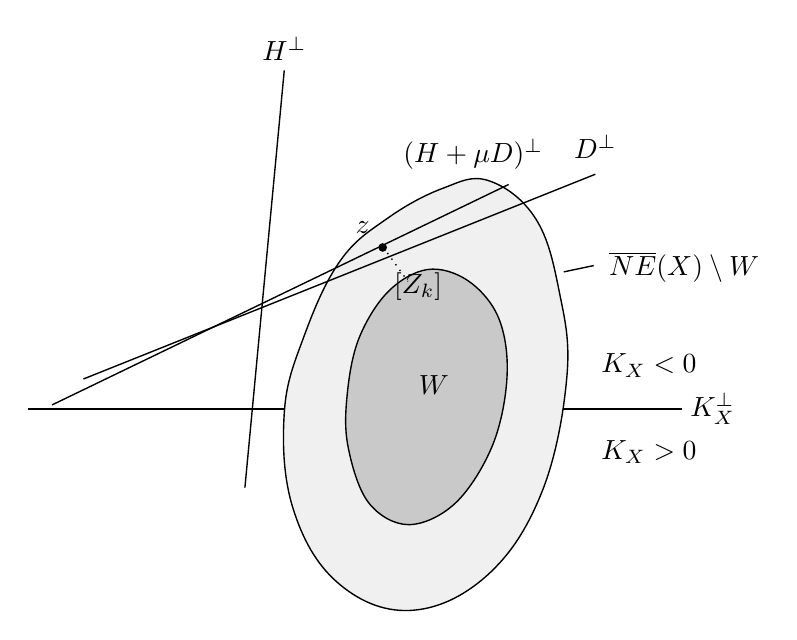
\begin{tikzpicture}[line width=0.5pt]
% 坐标轴
\draw (-2.20,0) -- (6.10,0);
\node[anchor=west] at (6.08,0.00) {$K_X^{\perp}$};
\node[anchor=west] at (4.95,0.55) {$K_X<0$};
\node[anchor=west] at (4.95,-0.55) {$K_X>0$};
% 外层区域 NE(X)\setminus W
\fill[gray!12] plot[smooth cycle, tension=0.65] coordinates
 {(1.05,-0.05) (1.30,0.92) (1.76,1.88) (2.36,2.42) (3.06,2.80)
  (3.64,2.90) (4.24,2.42) (4.54,1.50) (4.64,0.42) (4.32,-1.06)
  (3.62,-2.12) (2.64,-2.56) (1.72,-2.20) (1.16,-1.26)};
\draw plot[smooth cycle, tension=0.65] coordinates
 {(1.05,-0.05) (1.30,0.92) (1.76,1.88) (2.36,2.42) (3.06,2.80)
  (3.64,2.90) (4.24,2.42) (4.54,1.50) (4.64,0.42) (4.32,-1.06)
  (3.62,-2.12) (2.64,-2.56) (1.72,-2.20) (1.16,-1.26)};
% 内层区域 W
\fill[gray!42] plot[smooth cycle, tension=0.60] coordinates
 {(1.85,0.19) (2.00,0.90) (2.37,1.49) (2.87,1.77) (3.38,1.63)
  (3.77,1.16) (3.88,0.43) (3.70,-0.45) (3.23,-1.19) (2.63,-1.47)
  (2.12,-1.19) (1.86,-0.48)};
\draw plot[smooth cycle, tension=0.60] coordinates
 {(1.85,0.19) (2.00,0.90) (2.37,1.49) (2.87,1.77) (3.38,1.63)
  (3.77,1.16) (3.88,0.43) (3.70,-0.45) (3.23,-1.19) (2.63,-1.47)
  (2.12,-1.19) (1.86,-0.48)};
% 三条直线（共点于 P）
\coordinate (P) at (0.80,1.30);
\draw (1.05,4.30) -- (0.55,-1.00);
\draw (3.90,2.85) -- (-1.90,0.05);
\draw (5.00,2.98) -- (-1.50,0.38);
\node[above] at (1.05,4.30) {$H^{\perp}$};
\node[above] at (3.45,2.92) {$(H+\mu D)^{\perp}$};
\node[above] at (5.00,3.05) {$D^{\perp}$};
% 点 z 与 [Z_k]
\fill (2.30,2.05) circle (0.055);
\node[above left] at (2.26,2.10) {$z$};
\node at (2.75,1.55) {$[Z_k]$};
\draw[dotted] (2.36,1.98) -- (2.62,1.62);
% 区域标注
\node at (2.95,0.30) {$W$};
\node[anchor=west] (outs) at (5.05,1.80) {$\overline{NE}(X)\setminus W$};
\draw (4.98,1.82) -- (4.60,1.74);
\end{tikzpicture}
}
\figtitle{1.3}{定理 1.24 的证明中的闭锥 $W$ 与 $\overline{NE}(X)\setminus W$，以及超平面 $H^{\perp}$、$(H+\mu D)^{\perp}$、$D^{\perp}$（原书 p.30）}
\end{figure}

这些 $E_{i(k)}$ 与 $\{C_i\}$ 中的某一个数值等价，特别地 $(E_{i(k)}\cdot D)\ge0$。由此得到下列不等式。
\[ \frac{-(E_{i(k)}\cdot K_X)}{(E_{i(k)}\cdot H)}\ge\frac{-(E_{i(k)}\cdot K_X)}{(E_{i(k)}\cdot H+\mu'D)}\ge\frac{-(Z_k\cdot K_X)}{(Z_k\cdot H+\mu'D)}. \]
取正数 $M$ 足够大时，$MH+K_X$ 是丰富的。这蕴涵 $M\ge-(E_{i(k)}\cdot K_X)/(E_{i(k)}\cdot H)$，故下列不等式成立。
\[ M\ge\frac{-(E_{i(k)}\cdot K_X)}{(E_{i(k)}\cdot H)}\ge\frac{-(Z_k\cdot K_X)}{(Z_k\cdot H+\mu'D)}. \]
这里考虑 $i\to\infty$、$\mu'\to\mu$ 的极限。则
\[ M\ge\frac{-(Z_k\cdot K_X)}{(Z_k\cdot H+\mu'D)}\to\frac{-(z\cdot K_X)}{(z\cdot H+\mu D)}=\frac{-(z\cdot K_X)}{0}=+\infty. \]
这是矛盾的，故 $\overline{NE}(X)=W$ 得证。

% [Tutor Note: 这里取 μ 为最大的正数使 $H+\mu D$ 成为 nef，只用到 μ 是实数；有理性的精细信息留待以后的锥定理。矛盾来自 $-(z\cdot K_X)$ 为正而分母趋于 $0$，属于“极限处爆掉”的典型论证。]

固定 $H$ 与 $\epsilon$。若 $(C_i\cdot(K_X+\epsilon H))<0$，则

% [原文 p.31]
\[ (C_i\cdot H)\le\frac{-(C_i\cdot K_X)}{\epsilon}\le\frac{\dim X+1}{\epsilon} \]
成立，故由推论 1.19，这样的 $C_i$ 至多只有有限个。

记
\[ V_{H,\epsilon}:=\overline{NE}(X)_{(K_X+\epsilon H)\ge0}+\sum_{(C_i\cdot(K_X+\epsilon H))<0}\R_{\ge0}[C_i]. \]
$V_{H,\epsilon}$ 是闭锥，且包含 $W$。由于已证明 $W=\overline{NE}(X)$，锥定理的主张 (2) 得证。

最后证明定理 1.24(1) 的右端是闭的。这是关于 $\R^m$ 的锥的容易结果。首先注意下列一般事实。

$\R^m$ 的子集 $A$ 生成的凸锥的任意元 $\xi$，只要从 $A$ 中适当选取至多 $m$ 个元，就属于它们生成的凸锥。

证明时不妨设原点为中心的单位球面 $S^{m-1}$ 上含有 $A$。把 $S^{m-1}$ 上由 $A$ 生成的球面凸图形用 $A$ 的点为顶点的单体分割，则 $\xi$ 属于其中某个单体。该单体的顶点至多 $m$ 个。

取定理 1.24(1) 右端的元组成的收敛点列 $\xi_i$，记 $\xi:=\lim\xi_i$。把 $\xi_i$ 用 $\eta_i\in\overline{NE}(X)_{K_X\ge0}$ 与 $\rho(X)$ 个极射线的（可能为 $0$ 的）元 $\xi_{i,k}$（$k=1,\dots,\rho(X)$）表示为 $\xi_i=\eta_i+\sum_k\xi_{i,k}$。由推论 1.19(2)，$\{\eta_i\mid i>0\}$、$\{\xi_{i,k}\mid i>0\}$ 是紧点列。重取子列，可设它们都收敛。记 $\eta:=\lim\eta_i$、$\xi_k:=\lim\xi_{i,k}$。若 $(\xi_k\cdot K_X)\ge0$，则显然 $\xi_k\in\overline{NE}(X)_{K_X\ge0}$。另一方面，若 $(\xi_k\cdot K_X)<0$，则 $\xi_k$ 的近旁不聚集极射线，故 $\R_{\ge0}\xi_k=\R_{\ge0}\xi_{i,k}$（$i\gg0$）。因此
\[ \xi=\Bigl(\eta+\sum_{(\xi_k\cdot K_X)\ge0}\xi_k\Bigr)+\sum_{(\xi_k\cdot K_X)<0}\xi_k \]
属于右端。
\end{proof}

锥定理暗示了曲线锥的有趣结构，但这一新结构与以往研究的几何性质是否有关系并不清楚。关键在于极射线对应于簇的态射这一点。

\begin{definition}{1.25}
设 $X$ 为射影簇，$F\subset\overline{NE}(X)$ 为极锥面。当下列条件同时满足时，态射 $\operatorname{cont}_F:X\to Z$ 称为 $F$ 的收缩（contraction）：
% [原文 p.32]
\begin{enumerate}
\item 对不可约曲线 $C\subset X$，$\operatorname{cont}_F(C)$ 成为 $1$ 点的充要条件是 $[C]\in F$；
\item $(\operatorname{cont}_F)_*\cO_X=\cO_Z$。
\end{enumerate}
\end{definition}

% [Tutor Note: 收缩由极锥面唯一确定：条件 (1) 指定了被收缩的曲线集合，(2) 则要求非收缩方向的函数全部来自底空间，两者合起来正是 Stein 分解的唯一性。]

\begin{remark}{1.26}
如例 1.27 所见，一般来说并非任何极锥面都能收缩。毋宁说主要目的之一，是找出保证收缩态射 $\operatorname{cont}_F$ 存在的条件。低维非奇异情形在下一节处理，一般结果在第 3 章证明。

条件 (1) 作为集合决定了 $\operatorname{cont}_F$ 的纤维；(2) 则说 $\operatorname{cont}_F$ 是它自身的 Stein 分解（Stein factorization）。

（Stein 分解 [Har77, III.11.5]）Noether 概形的射影态射 $f:X\to Y$ 可唯一分解为纤维连通的射影态射 $f':X\to Y'$（满足 $f'_*\cO_X=\cO_{Y'}$）与有限态射 $g:Y'\to Y$ 的合成 $f=g\circ f'$。

因此，$\operatorname{cont}_F$ 由极锥面 $F$ 唯一决定。

设 $g:X\to Z$ 是到正规射影簇的态射，纤维连通。令 $F$ 为使 $g(C)$ 成为 $1$ 点的不可约曲线 $C$ 的类 $[C]$ 生成的子锥。则 $\operatorname{cont}_F=g$。于是，到正规射影簇的纤维连通的态射，全都是极锥面的收缩。
\end{remark}

\begin{example}[{[Zar62]}]{1.27}
在非奇异平面三次曲线 $D$ 上取 $12$ 个点 $p_1,\dots,p_{12}$，把以这些点为中心的爆破记为 $g:X\to\PP^2$，令 $C$ 为 $D$ 的双有理变换 $C=g^{-1}_*D$。此时 $C^2=-3$，且 $C$ 可通过到解析曲面 $Y$ 的解析态射 $f:X\to Y$ 压成一点（参看 [Gra62]）。然而，若 $12$ 个点处于一般位置，则 $Y$ 不是射影的。为看出这一点，设 $M$ 是 $Y$ 上任意的非平凡线丛。则 $f^*M$ 与除子 $g^*\cO_{\PP^2}(b)+\sum a_iE_i$ 线性等价，其中 $E_i$ 是点 $p_i$ 上的例外曲线。除子 $f^*M|_C$ 应线性等价于 $0$。于是得到 $D$ 上的线性等价关系 $\cO_D(b)+\sum a_ip_i\sim0$，而当 $p_i$ 取一般位置时这不成立。

但是，若 $12$ 个点 $p_i$ 是 $D$ 与四次曲线 $Q$ 的交点，则以 $C$ 为成分的四次曲线与 $Q$ 生成的线性系 $|M|$ 被双有理变换为自由线性系 $g^{-1}_*|M|$，它把 $f:X\to Y$ 实现为到射影空间的态射。
\end{example}

% [原文 p.33]
\section{曲面的极小模型}

\takeaway{本节的目的是从极射线的观点介绍曲面分类理论：对非奇异射影曲面，$K_X$-负极射线的收缩只有爆破、极小直纹曲面与 $\PP^2$ 三种；反复收缩即可得到极小模型。这一最单纯的设定是理解向高维推广的出发点。}

本节的目的是从极射线的观点介绍曲面的分类理论。这等于在非常单纯的设定下介绍极射线理论。之后回顾向三维簇的推广是怎样开始的。

本节中所有簇都假定定义在代数闭域 $k$ 上。

\begin{theoremp}{1.28}
设 $X$ 为非奇异射影曲面，$R\subset\overline{NE}(X)$ 是满足 $(R\cdot K_X)<0$ 的极射线。则收缩态射（定义 1.25）$\operatorname{cont}_R:X\to Z$ 存在，且表现为下列之一。

\begin{enumerate}
\item $Z$ 是非奇异曲面，$X$ 由 $Z$ 爆破闭点得到。又，$\rho(Z)=\rho(X)-1$。
\item $Z$ 是非奇异曲线，$X$ 是 $Z$ 上的极小直纹曲面。又，$\rho(X)=2$。
\item $Z$ 是 $1$ 点，$\rho(X)=1$，且 $-K_X$ 丰富。（实际上 $X\cong\PP^2$，但证明这一点很难。）
\end{enumerate}
\end{theoremp}

% [Tutor Note: 三种情形正对应 $(C^2)$ 的符号：正时为内点且 $-K_X$ 丰富，零时纤维全是 $\PP^1$，负时 $C$ 是 $(-1)$-曲线可爆破掉。读这一证明时先记住这个对应。]

\begin{proof}
取 $C\subset X$ 为使 $[C]\in R$ 的不可约曲线。下面说明上述 $3$ 种情形对应于 $(C^2)$ 的符号。

首先设 $(C^2)>0$。由推论 1.21 可知 $[C]$ 是 $\overline{NE}(X)$ 的内点。$[C]$ 同时是极射线的生成元，故 $N_1(X)\cong\R$。由假设 $(C\cdot K_X)<0$，$K_X$ 在 $\overline{NE}(X)\setminus\{0\}$ 上为负，故由定理 1.18，$-K_X$ 丰富。

其次考虑 $(C^2)=0$ 的情形。证明对适当的 $m\gg1$，$|mC|$ 给出收缩态射。由于 $C$ 有效，$m\gg1$ 时 $H^2(X,\cO(mC))=0$。由假设 $(K_X\cdot C)<0$，$m\gg1$ 时下列成立。
\[ h^0(X,\cO(mC))\ge\chi(X,\cO(mC))=\frac{-K_X\cdot C}{2}m+\chi(\cO_X)\ge2. \]
固定部分都是 $C$ 的倍数，故适当取 $m'>0$ 可使 $|m'C|$ 没有固定部分。又由 $(C^2)=0$，线性系 $|m'C|$ 的一般元与 $C$ 不相交，故 $|m'C|$ 没有基点。令 $\operatorname{cont}_R:X\to Z$ 为对应态射的 Stein 分解。

% [原文 p.34]
设 $\sum a_iC_i$ 是态射 $\operatorname{cont}_R$ 的任意纤维。则 $\sum a_i[C_i]=[C]\in R$。由于 $R$ 是极射线，由此对每个 $i$ 有 $[C_i]\in R$。于是得到 $(C_i^2)=0$ 与 $(C_i\cdot K_X)<0$。由伴随公式，这蕴涵 $C_i\cong\PP^1$ 与 $(C_i\cdot K_X)=-2$。因此
\[ -2=(C\cdot K_X)=\Bigl(\sum a_iC_i\cdot K_X\Bigr)=-2\sum a_i, \]
由此可知 $\sum a_iC_i$ 是不可约且既约的曲线，且与 $\PP^1$ 同构。于是 $X$ 是 $Z$ 上的极小直纹曲面。

最后设 $(C^2)<0$。由伴随公式可知 $C$ 是 $(-1)$-曲线，故由定理 1.28(1) 归结为定理 1.2。
\end{proof}

定理 1.28(2)--(3) 的情形已得到 $X$ 的结构定理。另一方面，定理 1.28(1) 的情形引入了新曲面 $Z$。我们可以对 $Z$ 应用定理 1.28，若可能还可继续下去。每一步 Picard 数都减少 $1$，故有限次反复后这一过程终止。由此得到下列结果。

\begin{theorem*}{1.29}
设 $X$ 为非奇异射影曲面。则存在由非奇异射影曲面与收缩态射组成的列
\[ X\to X_1\to\cdots\to X_n=X', \]
使 $X'$ 满足下列条件之一。

\begin{enumerate}
\item $K_{X'}$ 是 nef。
\item $X'$ 是曲线 $C$ 上的极小直纹曲面。
\item $X'\cong\PP^2$。
\end{enumerate}
\end{theorem*}

\begin{definition}{1.30}
若 $K_{X'}$ 是 nef（定理 1.29(1) 的情形），则称 $X'$ 为曲面 $X$ 的极小模型（minimal model）。此时对 $X$ 而言，定理 1.29 中总只发生 (1) 的情形，态射 $X\to X'$ 除同构外唯一。这可用后述的定义 3.50、定理 3.52(2) 证明。但本定义被（等价但表面上更一般的）定义 2.13 吸收，第 2 章以后不再使用，故不再深入。
\end{definition}

\par\medskip\noindent\textbf{概要 1.31}\quad 至此所述，曲面极小模型的构成法给出如下步骤。

% [原文 p.35]
\par\smallskip\noindent\textbf{步骤 0}\quad 从非奇异射影曲面 $X$ 出发。

\par\smallskip\noindent\textbf{步骤 1}\quad 若 $K_X$ 是 nef，则进入步骤 5。若 $K_X$ 不是 nef，则由锥定理可选 $K_X$-负的极射线 $R\subset\overline{NE}(X)$。

\par\smallskip\noindent\textbf{步骤 2}\quad 由定理 1.28，收缩态射 $\operatorname{cont}_R:X\to Z$ 存在。有两种情形。

\par\smallskip\noindent\textbf{步骤 3}\quad 若 $\dim Z=\dim X$，则把 $X$ 换成 $Z$，回到步骤 0。

\par\smallskip\noindent\textbf{步骤 4}\quad 若 $\dim Z<2=\dim X$，则由定理 1.28(2)--(3) 得到 $X$ 的结构定理。

\par\smallskip\noindent\textbf{步骤 5}\quad 若 $K_X$ 是 nef，则在此停止。这些曲面用其他方法研究。\hfill$\square$

森纲领的目的是对高维簇给出同样的构成法步骤。对应步骤 1 的部分是锥定理，而收缩可能性部分稍后证明。

下一步是把定理 1.28 的类似结果推广到高维簇。即使在 $\C$ 上的非奇异三维簇的情形，也会出现许多情形 [Mor82]。任意特征的代数闭域上的非奇异三维簇也有本质上相同的分类结果 [Kol91a]。[AW97] 对 $\C$ 上的非奇异四维簇的分类作了概述。

\begin{theorem}[{[Mor82]}]{1.32}
设 $X$ 为 $\C$ 上的三维非奇异射影簇，$\operatorname{cont}_R:X\to Y$ 为 $K_X$-负极射线 $R\subset\overline{NE}(X)$ 的收缩。则 $\operatorname{cont}_R$ 表现为下列之一。

\textbf{E}（例外型）\quad $\dim Y=3$，且 $\operatorname{cont}_R$ 是双有理的。例外曲面近旁的状况有下列 $5$ 种。

\par\smallskip\noindent\hspace{1.2em}\textbf{E1}\quad $\operatorname{cont}_R$ 是非奇异三维簇 $Y$ 沿非奇异曲线的爆破（之逆）。

\par\smallskip\noindent\hspace{1.2em}\textbf{E2}\quad $\operatorname{cont}_R$ 是非奇异三维簇 $Y$ 在 $1$ 点的爆破（之逆）。

\par\smallskip\noindent\hspace{1.2em}\textbf{E3}\quad $\operatorname{cont}_R$ 是三维簇 $Y$ 的通常 $2$ 重点的爆破（之逆）。局部解析地描述，通常 $2$ 重点由方程 $x^2+y^2+z^2+w^2=0$ 给出。

% [原文 p.36]
\par\smallskip\noindent\hspace{1.2em}\textbf{E4}\quad $\operatorname{cont}_R$ 是三维簇 $Y$ 的 $2$ 重点的爆破（之逆）。局部解析地描述，该 $2$ 重点由方程 $x^2+y^2+z^2+w^3=0$ 给出。

\par\smallskip\noindent\hspace{1.2em}\textbf{E5}\quad $\operatorname{cont}_R$ 把法丛（normal bundle）为 $\cO(-2)$ 的 $\PP^2$ 压成簇 $Y$ 的 $4$ 重点。该 $4$ 重点局部解析地由 $\C^3$ 的 $2$ 阶自同构 $(x,y,z)\mapsto(-x,-y,-z)$ 的商空间给出。

\textbf{C}（二次曲线丛（conic bundle））\quad $\dim Y=2$，态射 $\operatorname{cont}_R$ 的纤维都是平面二次曲线。（一般纤维当然非奇异。）

\textbf{D}（Del Pezzo 纤维空间（fibration））\quad $\dim Y=1$，态射 $\operatorname{cont}_R$ 的一般纤维是 Del Pezzo 曲面。

\textbf{F}（Fano 簇（Fano variety））\quad $\dim Y=0$，且 $-K_X$ 丰富。因此 $X$ 是 Fano 簇。
\end{theorem}

% [Tutor Note: E3、E4、E5 是进入三维后才首次出现的新现象，共同点是底 $Y$ 带奇点，因而不能对 $Y$ 再用定理 1.32；它们正是三维极小模型理论必须处理奇点的原因。]

情形 C 与情形 D 可看作极其令人满意的结构定理。情形 F 也许显得更不完全，但此处出现的三维 Fano 簇已被完全分类。详情请参看 [Isk80, Tau89, Muk95]。

情形 E1 与情形 E2 是定理 1.28(1) 的忠实类似，可对 $Y$ 再次应用定理 1.32。情形 E3、E4、E5 是进入三维后才首次出现的意外情形。这里 $Y$ 具有奇点，不能对 $Y$ 应用定理 1.32。

下一章概述森纲领或称极小模型纲领。它是概要 1.31 向高维的推广。在其过程中会遇到许多意外结果与未解决的问题。

\section{丰富性判别法}

\takeaway{本节补充 §1.3：先复习交点数的定义与基本性质，再证明中井--Moishezon 判别法（定理 1.37），并由此导出 Kleiman 判别法（定理 1.18）。核心工具是 Noether 归纳与 nef 除子的正性。}

本节补充 §1.3，是基本丰富性判别法（定理 1.18）与定理 1.44 的简短的入门。本书只把这些判别法应用于射影簇，故为使处理简单，往往只处理这一情形。详情请参看 [Har70, Kol96]。

% [原文 p.37]
这里把除子的交点数的基本部分略加复习。首先确定记号，然后大体解说交点数的定义方式，并列举本书所需的基本性质。

\begin{notation}{1.33}
$X$ 是域 $k$ 上的固有概形，$Z\subset X$ 是 $d$ 维闭子概形，$L_1,\dots,L_d$ 是 $X$ 上的 Cartier 除子。$(L_1\cdots L_d\cdot Z)$ 是除子 $L_1,\dots,L_d$ 在 $Z$ 上的相交数。若 $L_1=\cdots=L_d=L$，也可用 $(L^d\cdot Z)$ 这一记号。当 $Z=X$ 时，若不易产生误解，也可用 $(L_1\cdots L_d)$ 这一记号。\hfill$\square$
\end{notation}

\par\medskip\noindent\textbf{1.34}（交点数的定义）\quad 定义交点数至少有下列 $4$ 种手法。

（古典手法）设 $L_1,\dots,L_d$ 与 $Z$ 只在非奇异点相交，且各交点处的切空间独立。此时把 $(L_1\cdots L_d\cdot Z)$ 定为（$k$ 的代数闭包上的）交点数。由此可用线性性把交点数的定义推广到任意除子。详情参看 [Sha94, Chap. IV] 等。

（上同调手法）这一手法证明 Euler 示性数
\[ \chi(Z,\cO_Z(m_1L_1+\cdots+m_dL_d)) \]
是关于 $m_1,\dots,m_d$ 的至多 $d$ 次多项式（称为 Hilbert 多项式），并把 $m_1\cdots m_d$ 的系数定义为 $(L_1\cdots L_d\cdot Z)$。这是 [Kle66, Kol96] 的手法。

（一般交叉理论）首先定义 Cartier 除子与任意闭子概形的交叉。先让 $Z$ 与 $L_d$ 交叉，其交叉再与 $L_{d-1}$ 交叉，如此继续到 $L_1$，得到闭子概形。把其 $0$ 维部分的次数作为 $(L_1\cdots L_d\cdot Z)$ 的定义。详情参看 [Ful84, 2.3]、[Har77, I.7] 等。

（拓扑手法）若 $X$ 定义在 $\C$ 上，则 $\cO_X(L)$ 有第 $1$ Chern 类 $c_1(L)\in H^2(X,\Z)$，$Z\subset X$ 有基本类 $[Z]\in H_{2d}(X,\Z)$。若 $X$ 连通，则 $[\text{点}]\in H_0(X,\Z)$ 与点的位置取法无关，故令
\[ (L_1\cdots L_d\cdot Z)\cdot[\text{点}]:=(c_1(L_1)\cup\cdots\cup c_1(L_d))\cap[Z]. \]
详情参看 [GH78]。\hfill$\square$

% [Tutor Note: 四种定义各有适用场合：古典手法给几何直观，上同调手法便于计算示性数，交叉理论最一般，拓扑手法在复情形最简。后文用哪一条取决于需要。考试式地记四条定义没有意义，记住各自的用途即可。]

% [原文 p.38]
关于所有这些手法，需要确认的事项很多，各手法给出的定义都等价也并非显然，但我们不必深入到此。本书所需的交点数的基本性质，在下一命题中列举。若承认上述等价性，证明便容易，委之于上述文献。

\begin{proposition*}{1.35}
交点数具有下列性质。

\begin{enumerate}
\item 若 $X\supset Y\supset Z$，$L'_i$ 是 $Y$ 上的 Cartier 除子，且对所有 $i$ 有 $\cO_X(L_i)|_Y\cong\cO_Y(L'_i)$，则
\[ (L_1\cdots L_d\cdot Z)=(L'_1\cdots L'_d\cdot Z). \]
\item $(L_1\cdots L_d\cdot Z)$ 关于 $L_i$ 是对称且多重线性的。
\item 若 $X\subset\PP^N$ 且 $\cO_X(L)=\cO_X(1)$，则 $(L^d\cdot Z)=\deg Z$。
\item 若 $L_1\equiv0$，则 $(L_1\cdots L_d\cdot Z)=0$。
\item 若 $D\subset Z$ 是 Cartier 除子且 $\cO_X(L_d)|_Z\cong\cO_Z(D)$，则
\[ (L_1\cdots L_d\cdot Z)=(L_1\cdots L_{d-1}\cdot D). \]
\item 若 $Z,Z'$ 是整概形且 $f:Z'\to Z$ 双有理，则
\[ (L_1\cdots L_d\cdot Z)=(f^*L_1\cdots f^*L_d\cdot Z'). \]
\end{enumerate}
\end{proposition*}

使用下列形式的 Riemann--Roch 定理。

\begin{theorem*}{1.36}
设 $X$ 是域上的 $n$ 维固有概形，$L_1,\dots,L_r$ 是 $X$ 上的 Cartier 除子。此时 $\chi(X,\cO_X(k_1L_1+\cdots+k_rL_r))$ 是关于 $(k_1,\dots,k_r)$ 的至多 $n$ 次多项式，且
\[ \chi\Bigl(X,\cO_X\Bigl(\sum_{i=1}^r k_iL_i\Bigr)\Bigr)=\frac{\bigl(\bigl(\sum_{i=1}^r k_iL_i\bigr)^n\bigr)}{n!}+(\text{次数}<n) \]
成立。其中 $\bigl(\bigl(\sum k_iL_i\bigr)^n\bigr)$ 是上面定义的相交数。
\end{theorem*}

Riemann--Roch 定理（参看 [Har77, App. A]）决定全部系数，故这个 Riemann--Roch 弱定理是远比它弱的结果。用上同调手法证明定理 1.36 最为容易。归到 $L_i$ 全都十分丰富的情形，用关于 $\dim X$ 与 $r$ 的归纳法应用 [Har77, III.5, Ex.5.2.(a)] 的讨论即可。这一证明本质上与定理 1.37 的证明的步骤 1 的讨论相同。

% [Tutor Note: 弱 Riemann-Roch 只要求最高次项与相交数一致，低次项完全不管。正因如此它才能对任意固有概形成立；而完整 Riemann-Roch 需要 Todd 类，对奇异概形要困难得多。]
